\chapter{Teknik Laboratorium II: Sintesis dan Analisis dalam Praktik}\label{ch:b2:lab-techniques-2}

Sebuah reaksi Grignard gagal pada suatu Senin pagi: labunya telah dibilas
tetapi tidak dikeringkan, dan beberapa tetes air yang tersisa di dalamnya
merusak pereaksi itu begitu terbentuk. Ketika dijalankan lagi dengan alat
gelas yang dikeringkan dalam oven, di bawah nitrogen, dengan halida yang
ditambahkan tetes demi tetes ke dalam labu yang diaduk dan didinginkan,
reaksi yang sama berhasil. Kimianya tidak berubah; susunan alatnya yang
berubah. Bab ini membahas praktik yang mengubah reaksi di atas kertas
menjadi produk di dalam vial: mengendalikan reaksi, mencegah masuknya udara
dan air, mengolahnya, memurnikannya, dan membuktikan apa yang telah dibuat.

\begin{omfigure}
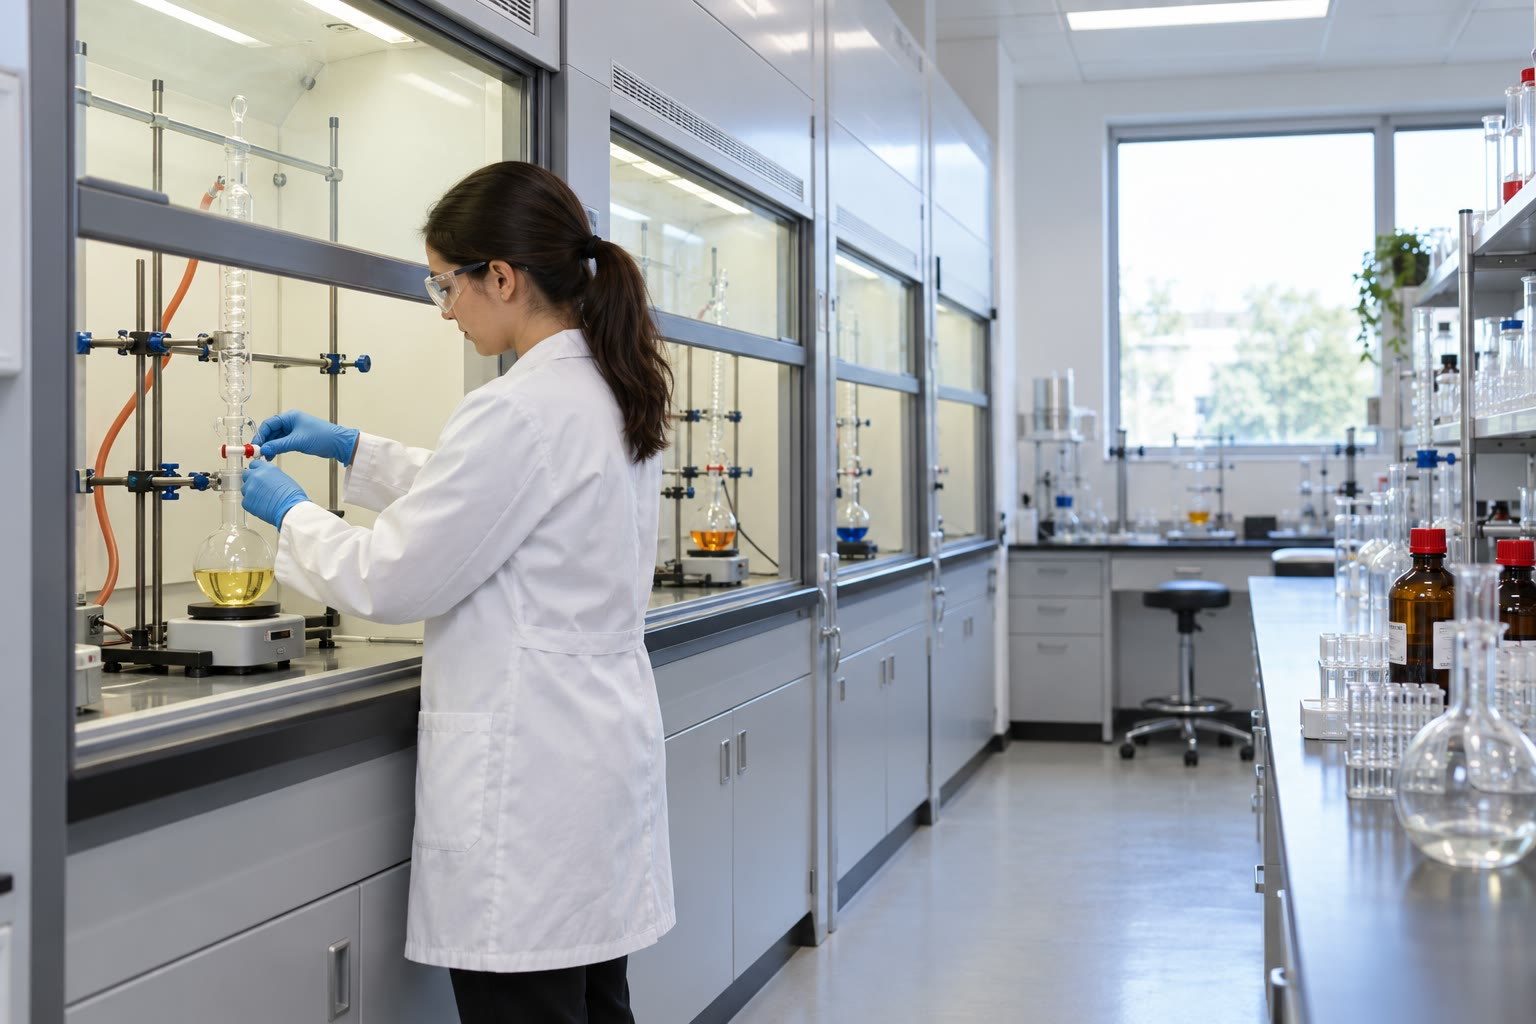
\includegraphics[width=0.56\linewidth]{images/book3/ai/b2-35-synthesis-lab.jpg}

{\small Sebuah laboratorium sintesis organik: reaksi-reaksi dijalankan di
dalam lemari asam, dengan labu-labu yang dijepit pada statif (ilustrasi).}
\end{omfigure}

\begin{recall}
Jilid Tahun 1: bahaya dan label GHS, ekstraksi, rekristalisasi, distilasi,
\omterm{def:b2:chromatography:principle}{kromatografi} lapis tipis dan $R_f$, titik leleh, pereaksi Grignard.
\Cref{ch:b2:reaction-enthalpy}: \omterm{def:b2:reaction-enthalpy:reaction-quantity}{entalpi reaksi} dan \omterm{def:b2:continuous-reactors:adiabatic-rise}{kenaikan suhu adiabatik}.
\Cref{ch:b2:chromatography},
\cref{ch:b2:structure-determination}, dan \cref{ch:b2:measurement-statistics}: analisis.
\end{recall}

\section{Menjalankan reaksi secara terkendali}

Reaksi di dalam labu melepaskan kalornya di tempat reaksi itu terjadi.
Kimiawan mengendalikan suhu dengan penangas (es dan air, es dan garam, es
kering dan aseton untuk suhu terendah), dengan refluks pelarut yang
mendidih, yang membatasi suhu pada titik didihnya sementara kondensor
mengembalikan uapnya, dan dengan laju penambahan pereaksi. Termometer di
bagian dalam, di dalam cairan alih-alih di dalam penangas, mengukur hal yang
penting.

\begin{proposition}[Akumulasi]\label{prop:b2:lab-techniques-2:accumulation}
Jika sebuah pereaksi ditambahkan lebih cepat daripada laju bereaksinya,
jumlah yang belum bereaksi $n_{\mathrm{acc}}$ terakumulasi. Seandainya
jumlah itu lalu bereaksi sekaligus, tanpa pendinginan, suhu campuran
berkapasitas kalor $C$ naik sebesar
\begin{equation*}
\Delta T_{\mathrm{ad}} = \frac{n_{\mathrm{acc}}\,|\Delta_rH|}{C}.
\end{equation*}
\end{proposition}

\begin{proof}
Reaksi $n_{\mathrm{acc}}$ melepaskan $n_{\mathrm{acc}}|\Delta_rH|$ pada
tekanan tetap (\cref{ch:b2:reaction-enthalpy}); tanpa pertukaran kalor,
seluruhnya menghangatkan campuran, seperti pada \omterm{def:b2:reaction-enthalpy:flame-temperature}{suhu nyala adiabatik}
(\cref{def:b2:reaction-enthalpy:flame-temperature}): $C\Delta T =
n_{\mathrm{acc}}|\Delta_rH|$.
\end{proof}

Bahayanya paling besar jika reaksi lambat dimulai, seperti yang sering
terjadi pada pembentukan pereaksi Grignard: halida yang ditambahkan sebelum
reaksi dimulai menumpuk, dan ketika reaksi akhirnya dimulai, reaksi itu
lepas kendali. Aturannya adalah menambahkan sebagian kecil, melihat reaksi
dimulai (penghangatan, kekeruhan, refluks yang lembut), dan baru kemudian
menambahkan sisanya dengan laju yang dapat diikuti oleh pendinginan.

\section{Kondisi kering dan atmosfer inert}

\begin{definition}[Atmosfer inert]\label{def:b2:lab-techniques-2:inert}
Sebuah reaksi dijalankan di bawah \emph{atmosfer inert}\index{atmosfer inert}
jika udara di dalam alat telah digantikan oleh gas yang tidak reaktif,
nitrogen atau argon, yang dijaga pada tekanan sedikit berlebih sehingga
udara tidak dapat masuk.
\end{definition}

Pereaksi organologam, hidrida logam, dan banyak katalis bereaksi dengan air
dan oksigen. Alat gelas dikeringkan dalam oven dan dirakit selagi hangat,
atau dipanaskan dengan api di bawah aliran gas; pelarut dibeli dalam
keadaan kering atau dikeringkan di atas pereaksi yang bereaksi dengan air;
cairan dipindahkan dengan semprit melalui sekat karet. Gas keluar melalui
penggelembung minyak, yang memperlihatkan alirannya dan mencegah udara
mengalir balik. Jalur Schlenk dan kotak sarung tangan, untuk senyawa yang
paling peka, dibahas dalam jilid Tahun 3.

\begin{omfigure}
\begin{tikzpicture}[lab/.style={font=\scriptsize, align=center}]
\fill[omDef!10] (-1.7,-0.3) rectangle (1.7,1.0);
\draw[om glass] (-1.7,1.2) -- (-1.7,-0.3) -- (1.7,-0.3) -- (1.7,1.2);
\foreach \x/\y in {-1.5/0.0,-1.45/0.55,1.3/0.05,1.3/0.6,-1.25/0.3,1.05/-0.15}{
  \draw[omDef!50, fill=white] (\x,\y) rectangle ++(0.18,0.18);}
\pic (f) at (0,0) {threeneck={0.35}{omThm!25}};
\pic[rotate=25] (d) at (f-l) {dropfunnel={0.5}{omMeth!20}};
\pic (c) at (f-c) {condenser};
\pic[rotate=-25] (t) at (0.0,0.42) {thermometer};
\pic (b) at (3.6,3.6) {bubbler};
\draw[thick, black!60] (0,6.25) -- (0,6.75) -- (3.25,6.75) -- (b-in);
\coordinate (dtop) at ($(f-l)+(-1.52,3.26)$);
\draw[thick, black!60] (dtop) -- ++(0,0.35) -- ++(-0.9,0) node[left, lab] {N$_2$};
\node[lab, anchor=north] at (0,-0.4) {penangas es};
\node[lab, anchor=east] at (-1.9,2.6) {corong\\penetes};
\node[lab, anchor=west] at (0.55,5.0) {kondensor};
\node[lab, anchor=west] at (1.75,2.6) {termometer\\(di dalam)};
\node[lab, anchor=north] at (3.6,3.45) {penggelembung (gas keluar)};
\end{tikzpicture}
\par\vspace{4pt}

{\small Reaksi di bawah nitrogen (skematis). Labu berleher tiga di dalam
penangas es, dengan termometer di dalam cairan; pereaksi ditambahkan dari
corong penyetara tekanan yang juga menjadi jalan masuk nitrogen; gas keluar
melalui kondensor dan penggelembung minyak.}
\end{omfigure}

\begin{method}[Menyiapkan reaksi kering di bawah nitrogen]\label{met:b2:lab-techniques-2:anhydrous}
\begin{enumerate}
  \item Keringkan alat gelas dalam oven dan rakitlah selagi panas, dengan
        melumasi atau memberi selongsong pada sambungan-sambungannya;
        pasanglah sekat atau corong penetes, kondensor, dan penggelembung.
  \item Aliri dengan nitrogen selama alat itu mendingin; pertahankan aliran
        yang lambat (satu gelembung setiap satu atau dua detik) sepanjang
        proses.
  \item Tambahkan padatan sebelum pengaliran gas, pelarut kering dan
        pereaksi cair dengan semprit atau kanula melalui sekat.
  \item Dinginkan atau panaskan sesuai rencana; mulailah penambahan dengan
        sebagian kecil dan periksalah bahwa reaksi dimulai sebelum
        melanjutkan.
\end{enumerate}
\end{method}

\section{Pengolahan}

\begin{definition}[Pengolahan]\label{def:b2:lab-techniques-2:work-up}
Yang disebut \emph{pengolahan}\index{pengolahan} sebuah reaksi adalah urutan
operasi, setelah reaksi, yang mengubah campuran reaksi menjadi produk
mentah: penghentian reaksi, ekstraksi dan pencucian, pengeringan,
penyaringan, dan penguapan pelarut.
\end{definition}

\begin{definition}[Ekstraksi asam--basa]\label{def:b2:lab-techniques-2:acid-base-extraction}
Yang disebut \emph{ekstraksi asam--basa}\index{ekstraksi asam--basa}
memisahkan senyawa-senyawa organik yang asam, basa, dan netral yang terlarut
dalam pelarut organik dengan mencuci larutan itu dengan asam atau basa
berair, yang mengubah satu kelas senyawa menjadi ion-ion yang berpindah ke
dalam air.
\end{definition}

\begin{proposition}[Siapa ke mana]\label{prop:b2:lab-techniques-2:acid-base-extraction}
Natrium hidrogenkarbonat berair (pH 8.3) mengekstraksi asam karboksilat
($\mathrm pK_a$ sekitar 4) tetapi tidak mengekstraksi fenol ($\mathrm pK_a$
sekitar 10), yang memerlukan natrium hidroksida; asam klorida encer
mengekstraksi amina yang asam konjugasinya mempunyai $\mathrm pK_a$ 4.6 atau
lebih; senyawa netral tetap berada di lapisan organik.
% ledger: ph:NaHCO3, pka:benzoic, pka:phenol, pka:anilinium
\end{proposition}

\begin{proof}
Sebuah spesies terutama berada dalam bentuk basanya jika $\mathrm{pH} > \mathrm pK_a$,
dan lebih dari 99~\% jika
$\mathrm{pH} > \mathrm pK_a + 2$. Pada pH 8.3, asam benzoat (4.2) lebih dari
99~\% berupa benzoat, sebuah ion yang tetap berada dalam air; fenol (9.99)
sekitar 2~\% berupa fenoksida ($10^{8.3 - 10.0}$) dan pada dasarnya tetap
berada di lapisan organik, tempat bentuk netralnya terpartisi. Dalam natrium
hidroksida (pH di atas 12) fenol diubah menjadi fenoksida. Dalam asam
klorida encer (pH sekitar 1), anilina (anilinium 4.6) lebih dari
99~\% berupa anilinium. Setiap ion, begitu berada dalam air, diperoleh
kembali dengan membalik pH ke arah sebaliknya, yang meregenerasi senyawa
netralnya, lalu mengekstraksinya lagi.
\end{proof}

\begin{omfigure}
\begin{tikzpicture}[x=1cm, y=1cm, st/.style={draw=black!70, rounded corners=2pt, fill=white,
  font=\scriptsize, align=center, inner sep=3pt, text width=3.0cm}, ar/.style={->, thick, black!70}]
\node[st, fill=omDef!10] (m) at (0,0) {asam benzoat, fenol,\\anilina, naftalena\\dalam etoksietana};
\node[st, fill=omThm!10] (a1) at (5.0,0) {berair: benzoat\\$\to$ HCl $\to$ asam benzoat};
\node[st] (o1) at (0,-1.6) {fenol, anilina,\\naftalena};
\node[st, fill=omThm!10] (a2) at (5.0,-1.6) {berair: fenoksida\\$\to$ HCl $\to$ fenol};
\node[st] (o2) at (0,-3.2) {anilina, naftalena};
\node[st, fill=omThm!10] (a3) at (5.0,-3.2) {berair: anilinium\\$\to$ NaOH $\to$ anilina};
\node[st, fill=omMeth!10] (o3) at (0,-4.8) {naftalena\\(keringkan, uapkan)};
\draw[ar] (m) -- node[above, font=\tiny] {cuci NaHCO$_3$} (a1);
\draw[ar] (m) -- (o1); \draw[ar] (o1) -- node[above, font=\tiny] {cuci NaOH} (a2);
\draw[ar] (o1) -- (o2); \draw[ar] (o2) -- node[above, font=\tiny] {cuci HCl} (a3);
\draw[ar] (o2) -- (o3);
\pic at (8.6,-3.6) {sepfunnel={omDef!25}{omThm!20}};
\node[font=\scriptsize, align=center] at (8.6,-4.0) {corong pisah};
\end{tikzpicture}
\par\vspace{4pt}

{\small Pemisahan asam--basa empat senyawa (\cref{prop:b2:lab-techniques-2:acid-base-extraction}).
Lapisan organik (kolom kiri) kehilangan satu kelas pada setiap pencucian;
setiap ekstrak berair (kanan) mengembalikan senyawanya ketika pH dibalik.}
\end{omfigure}

\begin{definition}[Zat pengering]\label{def:b2:lab-techniques-2:drying-agent}
Yang disebut \emph{zat pengering}\index{zat pengering} adalah garam
anhidrat, seperti magnesium sulfat atau natrium sulfat, yang mengikat air
yang terlarut dalam larutan organik sebagai air hidrat dan kemudian
disingkirkan dengan penyaringan.
\end{definition}

\begin{method}[Dari labu reaksi ke produk mentah]\label{met:b2:lab-techniques-2:work-up}
\begin{enumerate}
  \item Hentikan reaksi: musnahkan pereaksi reaktif yang tersisa dengan
        larutan berair yang sesuai, perlahan-lahan dan dengan pendinginan.
  \item Ekstraksi ke dalam pelarut organik; pisahkan lapisan-lapisannya
        (periksalah mana yang mana dengan menambahkan setetes air);
        ekstraksi lagi lapisan berairnya.
  \item Cucilah gabungan lapisan organik (asam, basa, lalu air garam pekat,
        larutan natrium klorida jenuh yang menyingkirkan sebagian besar air
        yang terlarut).
  \item Keringkan dengan \omterm{def:b2:lab-techniques-2:drying-agent}{zat pengering} sampai sebagian zat itu tetap
        lepas-lepas; saring.
  \item Singkirkan pelarut dengan penguap putar pada tekanan rendah;
        timbanglah produk mentahnya.
\end{enumerate}
\end{method}

\section{Pemurnian}

\begin{definition}[Kromatografi kilat]\label{def:b2:lab-techniques-2:flash}
Yang disebut \emph{kromatografi kilat}\index{kromatografi kilat} adalah
\omterm{def:b2:chromatography:principle}{kromatografi} kolom preparatif pada silika yang eluennya didorong melalui
kolom oleh tekanan gas yang ringan, sehingga pemisahan bahan berskala gram
hanya memakan waktu beberapa menit; eluennya dipilih dari \omterm{def:b2:chromatography:principle}{kromatografi}
lapis tipis pada silika yang sama.
\end{definition}

\begin{proposition}[Volume kolom]\label{prop:b2:lab-techniques-2:column-volumes}
Senyawa yang bergerak dengan $R_f$ pada pelat KLT keluar dari kolom dengan
silika dan eluen yang sama setelah sekitar $1/R_f$ volume kolom eluen.
\end{proposition}

\begin{proof}[Argumen]
Pada pelat, senyawa itu menempuh jarak $R_f$ kali jarak garis depan pelarut:
kecepatan rata-ratanya $R_f$
kali kecepatan eluen. Di dalam kolom, partisi yang sama memberikan rasio
kecepatan yang sama, sehingga senyawa itu memerlukan $1/R_f$ kali volume
eluen yang mengisi kolom (volume mati) untuk keluar; dalam bahasa
\cref{ch:b2:chromatography}, $R_f \approx 1/(1 + k)$. Senyawa pada $R_f = 0.25$
keluar setelah sekitar empat volume kolom, terpisah dengan baik dari senyawa
pada 0.5 (dua volume).
\end{proof}

\begin{omfigure}
\begin{tikzpicture}[lab/.style={font=\scriptsize, align=left, anchor=west}]
\pic (k) at (0,0) {chromcolumn={3.4}};
\node[lab] at (0.6,4.6) {eluen};
\node[lab] at (0.6,3.55) {pasir};
\node[lab] at (0.6,2.2) {unggun silika};
\foreach \i/\c in {0/white, 1/omThm!25, 2/omThm!25, 3/white, 4/omDef!25, 5/omDef!25, 6/white}{
  \pic at ({2.4+0.55*\i},-1.2) {testtube={0.45}{\c}};}
\node[font=\scriptsize] at (4.05,-1.6) {fraksi 1 sampai 7};
\pic at (7.6,-1.2) {tlcplate};
\foreach \j/\x in {2/7.15,3/7.45,5/7.75,6/8.05}{\node[font=\tiny] at (\x,-1.38) {\j};}
\fill[omThm] (7.45,0.95) circle (0.06); \fill[omThm] (7.15,0.95) circle (0.06);
\fill[omDef] (8.05,-0.05) circle (0.06); \fill[omDef] (7.75,-0.05) circle (0.06);
\node[font=\scriptsize, align=center] at (7.6,2.15) {KLT\\fraksi-fraksi};
\end{tikzpicture}
\par\vspace{4pt}

{\small \omterm{def:b2:lab-techniques-2:flash}{Kromatografi kilat} (skematis). Produk mentah dimuat di atas silika dan
dielusi; eluat ditampung dalam fraksi-fraksi; pelat KLT fraksi-fraksi itu
memperlihatkan tempat setiap senyawa keluar (di sini senyawa nonpolar yang
cepat dalam fraksi 2--3, yang lebih lambat dalam 5--6), dan fraksi-fraksi
yang murni digabungkan.}
\end{omfigure}

\begin{method}[Menjalankan kolom kilat]\label{met:b2:lab-techniques-2:flash}
\begin{enumerate}
  \item Pilihlah eluen dengan KLT: senyawa yang diinginkan pada $R_f$
        sekitar 0.25--0.35, sejauh mungkin dari pengotor-pengotornya.
  \item Kemaslah silika (sekitar 30 sampai 100 kali massa produk mentah)
        sebagai bubur atau dalam keadaan kering; tambahkan selapis pasir.
  \item Muatlah produk mentah dalam volume pelarut sekecil mungkin (atau
        teradsorpsi pada sedikit silika).
  \item Elusilah di bawah tekanan ringan; tampunglah fraksi-fraksi;
        periksalah dengan KLT; gabungkan yang murni dan uapkan.
\end{enumerate}
\end{method}

Cairan yang terurai di dekat titik didihnya didistilasi pada tekanan
rendah, tempat cairan itu mendidih pada suhu yang lebih rendah.

\begin{definition}[Distilasi pada tekanan rendah]\label{def:b2:lab-techniques-2:reduced-pressure}
Yang disebut \emph{distilasi pada tekanan rendah}\index{distilasi pada tekanan rendah}
dilakukan dalam alat yang dihubungkan ke pompa vakum melalui sebuah
manometer, pada tekanan yang membuat cairan mendidih pada suhu yang masih
dapat ditahannya.
\end{definition}

\begin{proposition}[Mendidih pada tekanan rendah]\label{prop:b2:lab-techniques-2:reduced-pressure}
Dengan $T_b$ suhu didih pada tekanan acuan $p^\circ$ dan $\Delta_{\mathrm{vap}}H$
yang dianggap tetap, suhu didih pada tekanan $p$ diberikan oleh
\begin{equation*}
\frac{1}{T} = \frac{1}{T_b} - \frac{R}{\Delta_{\mathrm{vap}}H}\ln\frac{p}{p^\circ}.
\end{equation*}
\end{proposition}

\begin{proof}
Cairan mendidih jika tekanan uapnya sama dengan tekanan di atasnya. Hubungan
Clausius--Clapeyron dari fisika,
$\mathrm d\ln p/\mathrm dT = \Delta_{\mathrm{vap}}H/(RT^2)$ untuk uap ideal dan volume cairan yang
dapat diabaikan, jika diintegralkan antara $(T_b, p^\circ)$ dan $(T, p)$ menjadi $\ln(p/p^\circ) =
-(\Delta_{\mathrm{vap}}H/R)(1/T - 1/T_b)$; penataan ulang menghasilkan hasilnya.
\end{proof}

\begin{omfigure}
\begin{tikzpicture}
\begin{axis}[width=0.72\linewidth, height=5.2cm, xmode=log, xmin=5, xmax=1100, ymin=0, ymax=190,
  xlabel={tekanan (\unit{mbar})}, ylabel={suhu didih (\unit{\degreeCelsius})},
  label style={font=\small}, tick label style={font=\scriptsize}, grid=major, grid style={black!10},
  legend style={font=\scriptsize, at={(0.02,0.98)}, anchor=north west}, legend cell align=left]
\addplot[omDef, thick] table[x=p, y=bromobenzene] {figdata/out/bachelor-2-vacuum-boiling.dat};
\addplot[omThm, thick] table[x=p, y=benzaldehyde] {figdata/out/bachelor-2-vacuum-boiling.dat};
\addplot[only marks, mark=o, mark size=2pt, omDef] coordinates {(7,27.75)};
\addplot[only marks, mark=o, mark size=2pt, omThm] coordinates {(13,61.85)};
\legend{bromobenzena, benzaldehida, terukur}
\end{axis}
\end{tikzpicture}

{\small Suhu didih terhadap tekanan (\cref{prop:b2:lab-techniques-2:reduced-pressure})
dengan entalpi penguapan dan titik didih dari NIST WebBook. Lingkaran-lingkaran
adalah titik didih terukur pada 7 dan \qty{13}{mbar}, yang tidak dipakai
dalam kurva: persamaan sederhana itu meleset hanya beberapa kelvin.
Menurunkan tekanan dari 1 bar menjadi \qty{20}{mbar} menurunkan titik didih
lebih dari
\qty{100}{K}.}
% figdata: bachelor-2/vacuum-boiling.py
% ledger: tb:bromobenzene, dvap:bromobenzene, tbp:bromobenzene.7mbar, tb:benzaldehyde, dvap:benzaldehyde, tbp:benzaldehyde.13mbar
\end{omfigure}

\section{Kemurnian dan identitas}

Sebuah produk diidentifikasi dengan membandingkan spektrum dan
tetapan-tetapan fisikanya dengan spektrum dan tetapan senyawa yang
diharapkan (\cref{ch:b2:structure-determination}); kemurniannya diukur
secara terpisah, karena sebuah produk dapat merupakan senyawa yang benar
namun tetap mengandung beberapa persen zat lain.

\begin{method}[Melaporkan kemurnian dan rendemen]\label{met:b2:lab-techniques-2:purity}
\begin{enumerate}
  \item Periksalah rentang leleh sebuah padatan (tajam dan dekat dengan
        nilai pustaka untuk senyawa murni) dan KLT-nya (satu bercak dalam
        dua eluen).
  \item Ukurlah kemurniannya: persen luas dalam GC atau HPLC (hanya
        perkiraan kecuali \omterm{def:b2:chromatography:quantitative}{faktor responsnya} diketahui,
        \cref{ch:b2:chromatography}), atau NMR proton kuantitatif, dengan
        membandingkan sebuah integral produk dengan integral setiap
        pengotor, atau dengan \omterm{def:b2:chromatography:quantitative}{standar internal} yang ditimbang.
  \item Ubahlah menjadi fraksi massa $w$ produk dalam bahan yang diisolasi.
  \item Laporkan rendemen yang dikoreksi untuk kemurnian: $\rho = w\,m/(n_{\mathrm{lim}}M)$,
        dengan $m$ massa yang diisolasi, $n_{\mathrm{lim}}$ jumlah pereaksi
        pembatas, dan $M$ massa molarnya.
\end{enumerate}
\end{method}

Untuk produk yang aktif secara optik, rotasi spesifik menambahkan
pemeriksaan kemurnian stereokimianya; kelebihan enansiomer dan
pengukurannya dibahas dalam jilid Tahun 3.

\begin{safety}{\ghs[5mm]{GHS02}\,\ghs[5mm]{GHS06}\,\ghs[5mm]{GHS07}\,\ghs[5mm]{GHS08}\,\ghs[5mm]{GHS09}}
Etoksietana dan oksolana sangat mudah terbakar dan membentuk peroksida
eksplosif selama penyimpanan; tidak boleh ada api di laboratorium, ujilah
botol-botol lama sebelum didistilasi. Bromobenzena mudah terbakar dan
beracun bagi kehidupan akuatik; serutan magnesium mudah terbakar. Alat gelas
vakum diperiksa dari retakan bintang dan diberi pelindung.
% ledger: ghs:ether, ghs:THF, ghs:bromobenzene, ghs:Mg, ghs:MgSO4
\end{safety}

\section{Latihan}

\begin{exercise}[$\star$]\label{exo:b2:lab-techniques-2:1}
Penangas apakah yang akan dipakai untuk reaksi yang dijalankan pada sekitar
\qty{0}{\degreeCelsius}, pada sekitar
\qty{-15}{\degreeCelsius}, dan pada \qty{-78}{\degreeCelsius}?
\end{exercise}

\begin{exercise}[$\star$]\label{exo:b2:lab-techniques-2:2}
Sebuah ekstraksi memakai diklorometana, yang lebih rapat daripada air. Lapisan manakah yang organik? Bagaimana memeriksanya?
\end{exercise}

\begin{exercise}[$\star$]\label{exo:b2:lab-techniques-2:3}
Bagaimana diketahui bahwa magnesium sulfat yang ditambahkan ke larutan eter sudah cukup?
\end{exercise}

\begin{exercise}[$\star$]\label{exo:b2:lab-techniques-2:4}
Dalam heksana--etil asetat 4\,:\,1, sebuah produk mempunyai $R_f = 0.65$ dan
sebuah pengotor 0.75. Apa yang perlu diubah untuk sebuah kolom, dan ke arah
mana?
\end{exercise}

\begin{exercise}[$\star\star$]\label{exo:b2:lab-techniques-2:5}
Tuliskan urutan pencucian yang memisahkan asam benzoat, fenol, anilina, dan
naftalena dari larutan eter, dengan membenarkan masing-masing dengan sebuah
$\mathrm pK_a$, dan bagaimana setiap senyawa diperoleh kembali.
\end{exercise}

\begin{exercise}[$\star\star$]\label{exo:b2:lab-techniques-2:6}
Perkirakan suhu didih bromobenzena dan benzaldehida pada \qty{20}{mbar}.
\end{exercise}

\begin{exercise}[$\star\star$]\label{exo:b2:lab-techniques-2:7}
Selama sebuah penambahan, \qty{0.050}{mol} pereaksi telah terakumulasi
tanpa bereaksi. Dengan $\Delta_rH =
\qty{-200}{kJ/mol}$ dan kapasitas kalor campuran \qty{400}{J/K} (data
latihan), kenaikan suhu berapakah yang dapat menyusul?
\end{exercise}

\begin{exercise}[$\star\star$]\label{exo:b2:lab-techniques-2:8}
Sebuah rekaman HPLC memperlihatkan produk pada 96.0~\% luas total. Mengapa
angka itu belum merupakan kemurnian massa? Spektrum proton sampel yang sama
memperlihatkan singlet produk (1H) dengan integral 1.00 dan singlet pengotor
(3H) dengan integral 0.12; produk \qty{200}{g/mol}, pengotor
\qty{100}{g/mol} (data latihan). Hitunglah fraksi massa produk.
\end{exercise}

\begin{exercise}[$\star\star$]\label{exo:b2:lab-techniques-2:9}
Diperoleh \qty{4.10}{g} sebuah produk (\qty{164}{g/mol}) dengan kemurnian
95.0~\% (massa) dari \qty{0.0300}{mol} pereaksi pembatas. Hitunglah
rendemennya, tanpa koreksi dan dengan koreksi.
\end{exercise}

\begin{exercise}[$\star\star\star$]\label{exo:b2:lab-techniques-2:10}
Sebuah reaksi Grignard menghasilkan benzena dan hampir tidak ada alkohol
setelah penambahan aldehida. Daftarlah penyebab-penyebab yang mungkin dan
cara menghindari masing-masing.
\end{exercise}

\begin{exercise}[$\star\star\star$]\label{exo:b2:lab-techniques-2:11}
Pada peningkatan skala, \qty{1.00}{mol} sebuah halida bereaksi dengan
$\Delta_rH = \qty{-270}{kJ/mol}$ dalam reaktor yang pendinginannya paling
banyak mengeluarkan \qty{150}{W} (data latihan). Berapa waktu penambahan
aman yang terpendek? Apa yang terjadi jika penambahannya lebih cepat?
\end{exercise}

\begin{exercise}[$\star\star\star$]\label{exo:b2:lab-techniques-2:12}
Sebuah padatan mentah seberat \qty{13.0}{g} dapat dimurnikan dengan
rekristalisasi (satu tahap, perolehan kembali 80~\%, kemurnian
99~\%) atau dengan \omterm{def:b2:lab-techniques-2:flash}{kromatografi kilat} (perolehan kembali 95~\%, kemurnian
99.5~\%, pelarut \qty{1.5}{L}) (data latihan). Bandingkan kedua jalur itu.
\end{exercise}

\section{Soal: Reaksi Grignard yang Dikerjakan dengan Benar}

\begin{problem}[{Soal akhir pekan --- bahaya dan susunan alat yang kering,
penambahan terkendali dan bahaya akumulasi, pengolahan, pemurnian dengan
kromatografi kilat, dan rendemen yang dikoreksi untuk kemurnian}]
\label{pb:b2:lab-techniques-2:1}
Data latihan. Fenilmagnesium bromida dibuat dari \qty{15.7}{g} bromobenzena
dan \qty{2.67}{g} serutan magnesium dalam etoksietana kering, lalu
\qty{9.55}{g} benzaldehida ditambahkan; \omterm{def:b2:lab-techniques-2:work-up}{pengolahan} dengan amonium klorida
berair menghasilkan difenilmetanol. Pembentukan pereaksi: $\Delta_rH =
\qty{-270}{kJ/mol}$; kapasitas kalor campuran \qty{170}{J/K}; mulai pada
\qty{20}{\degreeCelsius}. KLT
(heksana--etil asetat 9\,:\,1): bifenil $R_f = 0.85$, difenilmetanol 0.25.
Diisolasi setelah kolom:
\qty{12.50}{g}. NMR proton bahan ini: singlet \ce{CH(OH)} (1H) berintegral
1.00, daerah \omterm{def:b2:huckel:aromatic}{aromatik} 10.90. Massa molar (\unit{g/mol}): bromobenzena
157.01, benzaldehida 106.12, difenilmetanol
184.24, bifenil 154.21; Mg 24.305.
% ledger: ghs:ether, ghs:bromobenzene, ghs:Mg, ghs:benzaldehyde, ghs:NH4Cl, ghs:biphenyl, ghs:benzhydrol, tb:ether, aw:Mg, aw:C, aw:H, aw:Br, aw:O, nmr:biphenyl

\medskip
\noindent\textbf{Bagian I --- Bahaya dan susunan alat.}
\begin{enumerate}
  \item Sebutkan bahaya utama etoksietana, bromobenzena, dan magnesium.
  \item Tuliskan reaksi fenilmagnesium bromida dengan air, dan jelaskan
        alasan alat gelas dikeringkan dalam oven.
  \item Mengapa bekerja di bawah nitrogen?
  \item Apa yang diperlihatkan oleh penggelembung, dan apa yang dicegahnya?
  \item Mengapa etoksietana merupakan pelarut yang baik di sini?
  \item Hitunglah jumlah bromobenzena dan magnesium. Manakah yang berlebih?
\end{enumerate}

\medskip
\noindent\textbf{Bagian II --- Penambahan terkendali.}
\begin{enumerate}[resume]
  \item Berapa kalor yang dilepaskan oleh pembentukan pereaksi secara sempurna?
  \item Mengapa bromobenzena ditambahkan tetes demi tetes?
  \item Reaksinya lambat dimulai, dan 20~\% bromobenzena telah ditambahkan
        sebelum reaksi dimulai. Berapa kalor yang kemudian dapat dilepaskan
        sekaligus?
  \item Hitunglah \omterm{def:b2:continuous-reactors:adiabatic-rise}{kenaikan suhu adiabatiknya}.
  \item Bandingkan suhu akhirnya dengan titik didih etoksietana. Apa yang terjadi?
  \item Bagaimana penambahan itu seharusnya dilakukan?
\end{enumerate}

\medskip
\noindent\textbf{Bagian III --- Penambahan aldehida dan \omterm{def:b2:lab-techniques-2:work-up}{pengolahan}.}
\begin{enumerate}[resume]
  \item Tuliskan reaksi dengan benzaldehida dan kenalilah pereaksi pembatasnya.
  \item Mengapa reaksi dihentikan dengan amonium klorida alih-alih asam kuat?
  \item Lapisan manakah yang organik di dalam corong pisah?
  \item Untuk apa pencucian dengan air garam pekat?
  \item Bagaimana larutan itu dikeringkan, dan bagaimana pelarutnya disingkirkan?
  \item Bifenil adalah produk samping utama. Bagaimana bifenil terbentuk,
        dan apa yang mendukung pembentukannya?
\end{enumerate}

\medskip
\noindent\textbf{Bagian IV --- Pemurnian dan kemurnian.}
\begin{enumerate}[resume]
  \item Senyawa manakah yang lebih dahulu keluar dari kolom?
  \item Setelah berapa volume kolom masing-masing keluar?
  \item Dari integral NMR, hitunglah rasio mol bifenil terhadap alkohol dalam
        bahan yang diisolasi.
  \item Hitunglah fraksi massa difenilmetanol.
  \item Hitunglah massa difenilmetanol murni.
  \item Hitunglah massa teoretisnya.
  \item Hitunglah rendemen tanpa koreksi untuk kemurnian.
  \item Nyatakan rendemen yang dikoreksi untuk kemurnian.
\end{enumerate}
\end{problem}
